%%%%%%%% ICML 2021 EXAMPLE LATEX SUBMISSION FILE %%%%%%%%%%%%%%%%%

\documentclass{article}

% Recommended, but optional, packages for figures and better typesetting:
\usepackage{microtype}
\usepackage{graphicx}
\usepackage{subfigure}
\usepackage{booktabs} % for professional tables
\usepackage{lipsum}

% hyperref makes hyperlinks in the resulting PDF.
% If your build breaks (sometimes temporarily if a hyperlink spans a page), 
% please comment out the following usepackage line and replace
% \usepackage{icml2021} with \usepackage[nohyperref]{icml2021} above.
\usepackage{hyperref}

% Attempt to make hyperref and algorithmic work together better:
\newcommand{\theHalgorithm}{\arabic{algorithm}}

% Use the following line for the initial blind version submitted for review:
% \usepackage{icml2021}

% If accepted, instead use the following line for the camera-ready submission:
\usepackage[accepted]{icml2021}


% The \icmltitle you define below is probably too long as a header.
% Therefore, a short form for the running title is supplied here:
\icmltitlerunning{Submission and Formatting Instructions for ICML 2021}

\begin{document}

\twocolumn[
    \icmltitle{GPT2PPO: Auto Regressive Proximal Policy Optimization}

    % It is OKAY to include author information, even for blind
    % submissions: the style file will automatically remove it for you
    % unless you've provided the [accepted] option to the icml2021
    % package.

    % List of affiliations: The first argument should be a (short)
    % identifier you will use later to specify author affiliations
    % Academic affiliations should list Department, University, City, Region, Country
    % Industry affiliations should list Company, City, Region, Country

    % You can specify symbols, otherwise they are numbered in order.
    % Ideally, you should not use this facility. Affiliations will be numbered
    % in order of appearance and this is the preferred way.
    \icmlsetsymbol{equal}{*}

    \begin{icmlauthorlist}
        \icmlauthor{Andrei Cozma}{equal,utk}
        \icmlauthor{Hunter Price}{equal,utk}
    \end{icmlauthorlist}

    \icmlaffiliation{utk}{University of Tennessee, Knoxville, TN, USA}

    \icmlcorrespondingauthor{Andrei Cozma}{acozma@vols.utk.edu}
    \icmlcorrespondingauthor{Hunter Price}{hprice7@vols.utk.edu}
    % \icmlcorrespondingauthor{Eee Pppp}{ep@eden.co.uk}

    % You may provide any keywords that you
    % find helpful for describing your paper; these are used to populate
    % the "keywords" metadata in the PDF but will not be shown in the document
    \icmlkeywords{Reinforcement Learning, RL}

    \vskip 0.3in
]

% this must go after the closing bracket ] following \twocolumn[ ...

% This command actually creates the footnote in the first column
% listing the affiliations and the copyright notice.
% The command takes one argument, which is text to display at the start of the footnote.
% The \icmlEqualContribution command is standard text for equal contribution.
% Remove it (just {}) if you do not need this facility.

%\printAffiliationsAndNotice{}  % leave blank if no need to mention equal contribution
\printAffiliationsAndNotice{\icmlEqualContribution} % otherwise use the standard text.
% \printAffiliations
%%%%%%%%%%%%%%%%%%%%%%%%%%%%%%%%%%%%%%%%%%%%%%%%%%%%%%%%%%%%%%%%%%%%%%%%%%%%%%%
%% EXAMPLES:
%%%%%%%%%%%%%%%%%%%%%%%%%%%%%%%%%%%%%%%%%%%%%%%%%%%%%%%%%%%%%%%%%%%%%%%%%%%%%%%

%%%%%%%%%%%%%%%%%%%%%%%%%%%%%%%%%%%%%%%%
%% EXAMPLE FIGURE:
%%%%%%%%%%%%%%%%%%%%%%%%%%%%%%%%%%%%%%%%
% \begin{figure}[ht]
%     \vskip 0.2in
%     \begin{center}
%         \centerline{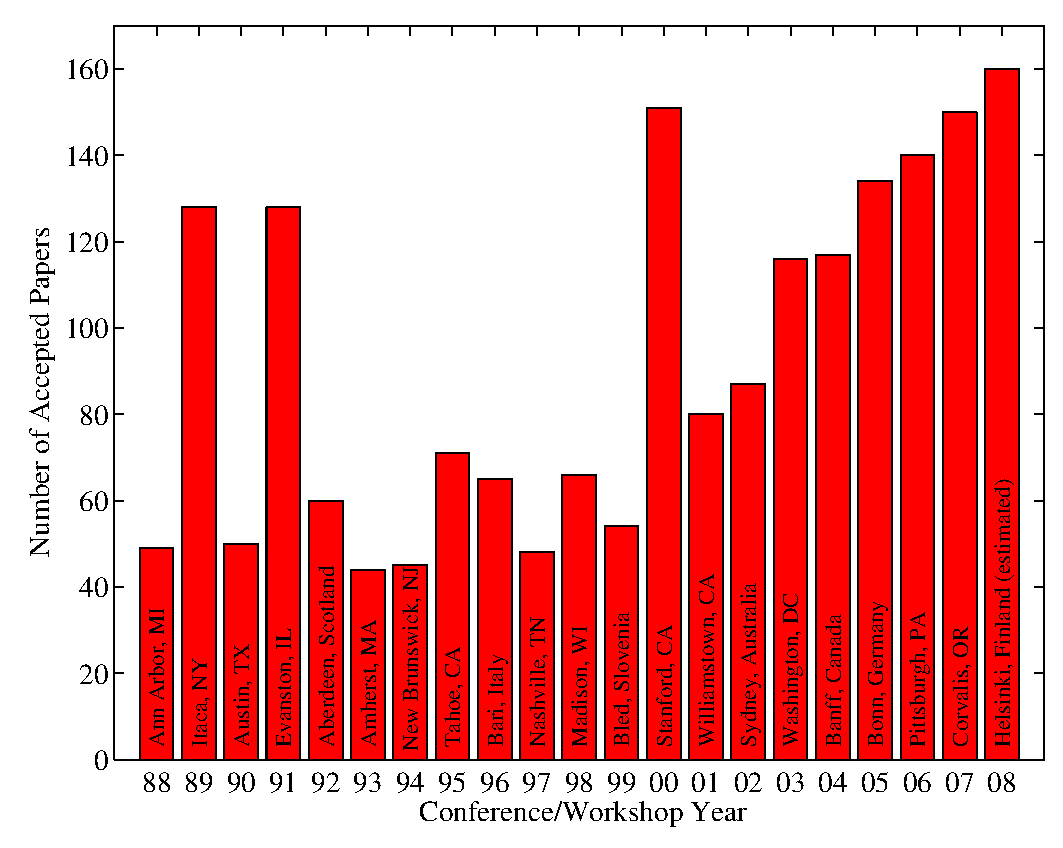
\includegraphics[width=\columnwidth]{icml_numpapers}}
%         \caption{Historical locations and number of accepted papers for International
%             Machine Learning Conferences (ICML 1993 -- ICML 2008) and International
%             Workshops on Machine Learning (ML 1988 -- ML 1992). At the time this figure was
%             produced, the number of accepted papers for ICML 2008 was unknown and instead
%             estimated.}
%         \label{icml-historical}
%     \end{center}
%     \vskip -0.2in
% \end{figure}
%
%
%%%%%%%%%%%%%%%%%%%%%%%%%%%%%%%%%%%%%%%%
%% EXAMPLE ALGORITHM:
%%%%%%%%%%%%%%%%%%%%%%%%%%%%%%%%%%%%%%%%
% \begin{algorithm}[tb]
%     \caption{Bubble Sort}
%     \label{alg:example}
%     \begin{algorithmic}
%         \STATE {\bfseries Input:} data $x_i$, size $m$
%         \REPEAT
%         \STATE Initialize $noChange = true$.
%         \FOR{$i=1$ {\bfseries to} $m-1$}
%         \IF{$x_i > x_{i+1}$}
%         \STATE Swap $x_i$ and $x_{i+1}$
%         \STATE $noChange = false$
%         \ENDIF
%         \ENDFOR
%         \UNTIL{$noChange$ is $true$}
%     \end{algorithmic}
% \end{algorithm}
%
%
%%%%%%%%%%%%%%%%%%%%%%%%%%%%%%%%%%%%%%%%
%% EXAMPLE TABLE:
% Note use of \abovespace and \belowspace to get reasonable spacing
% above and below tabular lines.
%%%%%%%%%%%%%%%%%%%%%%%%%%%%%%%%%%%%%%%%
% \begin{table}[t]
%     \caption{Classification accuracies for naive Bayes and flexible
%         Bayes on various data sets.}
%     \label{sample-table}
%     \vskip 0.15in
%     \begin{center}
%         \begin{small}
%             \begin{sc}
%                 \begin{tabular}{lcccr}
%                     \toprule
%                     Data set  & Naive         & Flexible      & Better?  \\
%                     \midrule
%                     Breast    & 95.9$\pm$ 0.2 & 96.7$\pm$ 0.2 & $\surd$  \\
%                     Cleveland & 83.3$\pm$ 0.6 & 80.0$\pm$ 0.6 & $\times$ \\
%                     Glass2    & 61.9$\pm$ 1.4 & 83.8$\pm$ 0.7 & $\surd$  \\
%                     Credit    & 74.8$\pm$ 0.5 & 78.3$\pm$ 0.6 &          \\
%                     Horse     & 73.3$\pm$ 0.9 & 69.7$\pm$ 1.0 & $\times$ \\
%                     Meta      & 67.1$\pm$ 0.6 & 76.5$\pm$ 0.5 & $\surd$  \\
%                     Pima      & 75.1$\pm$ 0.6 & 73.9$\pm$ 0.5 &          \\
%                     Vehicle   & 44.9$\pm$ 0.6 & 61.5$\pm$ 0.4 & $\surd$  \\
%                     \bottomrule
%                 \end{tabular}
%             \end{sc}
%         \end{small}
%     \end{center}
%     \vskip -0.1in
% \end{table}
%
%
%%%%%%%%%%%%%%%%%%%%%%%%%%%%%%%%%%%%%%%%%%%%%%%%%%%%%%%%%%%%%%%%%%%%%%%%%%%%%%%
%%%%%%%%%%%%%%%%%%%%%%%%%%%%%%%%%%%%%%%%%%%%%%%%%%%%%%%%%%%%%%%%%%%%%%%%%%%%%%%

%%%%%%%%%%%%%%%%%%%%%%%%%%%%%%%%%%%%%%%%%%%%%%%%%%%%%%%%%%%%%%%%%%%%%%%%%%%%%%%
%% PROJECT OVERVIEW:
%%%%%%%%%%%%%%%%%%%%%%%%%%%%%%%%%%%%%%%%%%%%%%%%%%%%%%%%%%%%%%%%%%%%%%%%%%%%%%%
% The goal of this project is for you to further explore a certain subject that we covered
% in class or a new subject related to it (based on some previous work). This is an open
% project in a sense that you will propose the problem you would like to work on and the
% solution you are planning use. Your main goal should be to explore the characteristics of
% your problem/solution under the reinforcement learning framework
%%%%%%%%%%%%%%%%%%%%%%%%%%%%%%%%%%%%%%%%%%%%%%%%%%%%%%%%%%%%%%%%%%%%%%%%%%%%%%%
%%%%%%%%%%%%%%%%%%%%%%%%%%%%%%%%%%%%%%%%%%%%%%%%%%%%%%%%%%%%%%%%%%%%%%%%%%%%%%%

%%%%%%%%%%%%%%%%%%%%%%%%%%%%%%%%%%%%%%%%%%%%%%%%%%%%%%%%%%%%%%%%%%%%%%%%%%%%%%%
%% REPORT INSTRUCTIONS
%%%%%%%%%%%%%%%%%%%%%%%%%%%%%%%%%%%%%%%%%%%%%%%%%%%%%%%%%%%%%%%%%%%%%%%%%%%%%%%
%1. Introduction(5%)
%In this section you should discuss the question you are planning to investigate. Make
%sure to describe the problem clearly, and how you are planning to solve it. Also, clarify
%what your new contribution is (as opposed to previous works).
%2. Previous Work(5%)
%Discuss the previous work you are using as a starting point/reference. If you are
%working on a different domain include work that works on the same or similar domain.
%If you are using a new method, discuss other works which use similar methods. Note
%that you can use both academic papers in addition to online articles. Make sure to cite
%all sources.
%3. Domain Problem(5%)
%Describe the problem you are working on including the rules, goals, etc. Assume that
%the reader has not been introduced to this domain problem previously. Then describe
%how you frame it as an MDP, including: state space, action space and reward structure.
%If you are examining different options describe them all. Feel free to add diagrams to
%clarify.
%3
%4. Reinforcement Learning Methods(5%)
%Describe the reinforcement method/methods you are planning to use in this work. This
%should give the background for the methods. If you are comparing multiple ones, make
%sure to describe them all. Feel free to add diagrams and equations to clarify.
%5. Code Design(5%)
%Describe the general structure of your code including functions, classes, and data struc-
%tures used. If you are using code written by someone else make sure to cite it and
%emphasize the parts that you have written yourself.
%6. Results Analysis(40%)
%Present the results which answer your hypothesis questions. These should include dif-
%ferent graphs which clarify the answer and examine different aspects of your solution.
%Make sure to carefully describe how your experiments were conducted (how many runs,
%how it was initialized, etc. This section is the most important, and will be evaluated
%both on presentation and correctness.
%7. Conclusion(5%)
%What have you achieved in this project? What have you learned?
%An appendix describing which part of the project each team member was in charge of.
%%%%%%%%%%%%%%%%%%%%%%%%%%%%%%%%%%%%%%%%%%%%%%%%%%%%%%%%%%%%%%%%%%%%%%%%%%%%%%%
%%%%%%%%%%%%%%%%%%%%%%%%%%%%%%%%%%%%%%%%%%%%%%%%%%%%%%%%%%%%%%%%%%%%%%%%%%%%%%%


%%%%%%%%%%%%%%%%%%%%%%%%%%%%%%%%%%%%%%%%%%%%%%%%%%%%%%%%%%%%%%%%%%%%%%%%%%%%%%%%%%%%%%%%%%%%%%%%%%%%%%%%%%%
%%%%%%%%%%%%%%%%%%%%%%%%%%%%%%%%%%%%%%%%%%%%%%%%%%%%%%%%%%%%%%%%%%%%%%%%%%%%%%%%%%%%%%%%%%%%%%%%%%%%%%%%%%%
%Introduction(5%)
%In this section you should discuss the question you are planning to investigate. Make
%sure to describe the problem clearly, and how you are planning to solve it. Also, clarify
%what your new contribution is (as opposed to previous works).

\section{Introduction}
\label{sec:introduction}
In this project we explore the use of transformers in the context of Reinforcement Learning. The majority of theoretical works 
assume that problems follow a Markovian process, which is not always the case. Some problems need the contxt of previous states and actions
to make an informed decision on the next decision. As a result, we propose an addition to the basic Proximal Policy Optimization (PPO) algorithm
by using the Generative Pre-trained Transformer 2 (GPT2) model as the encoder for the critic network. This will allow the critic network to
take into account the context of previous states and actions as well as apply attention to past states and actions that may be important. 
We will test this model on the LunarLander-v2 and Acrobot-v1 OpenAi Gym environments with discrete action spaces and compare it to the original PPO algorithm. 
Additionally we will test the model on BipedalWalker-v3 with continuous action spaces and compare it to the original PPO algorithm.


%%%%%%%%%%%%%%%%%%%%%%%%%%%%%%%%%%%%%%%%%%%%%%%%%%%%%%%%%%%%%%%%%%%%%%%%%%%%%%%%%%%%%%%%%%%%%%%%%%%%%%%%%%%
%%%%%%%%%%%%%%%%%%%%%%%%%%%%%%%%%%%%%%%%%%%%%%%%%%%%%%%%%%%%%%%%%%%%%%%%%%%%%%%%%%%%%%%%%%%%%%%%%%%%%%%%%%%
%Previous Work(5%)
%Discuss the previous work you are using as a starting point/reference. If you are
%working on a different domain include work that works on the same or similar domain.
%If you are using a new method, discuss other works which use similar methods. Note
%that you can use both academic papers in addition to online articles. Make sure to cite
%all sources.

\section{Previous Work}
\label{sec:previous-work}

% PPO citation - \cite{schulman2017proximal}
% Decision Transformer citation - \cite{chen2021decision}
% GPT2 citation - \cite{radford2019language}
% Wandb citation - \cite{wandb}

%%%%%%%%%%%%%%%%%%%%%%%%%%%%%%%%%%%%%%%%%%%%%%%%%%%%%%%%%%%%%%%%%%%%%%%%%%%%%%%%%%%%%%%%%%%%%%%%%%%%%%%%%%%
%%%%%%%%%%%%%%%%%%%%%%%%%%%%%%%%%%%%%%%%%%%%%%%%%%%%%%%%%%%%%%%%%%%%%%%%%%%%%%%%%%%%%%%%%%%%%%%%%%%%%%%%%%%
%Domain Problem(5%)
%Describe the problem you are working on including the rules, goals, etc. Assume that
%the reader has not been introduced to this domain problem previously. Then describe
%how you frame it as an MDP, including: state space, action space and reward structure.
%If you are examining different options describe them all. Feel free to add diagrams to
%clarify.
\section{Background}
\label{sec:background}

All of the environments used in this project are from the OpenAI Gym library \cite{brockman2016openai}. The environments are described below.

\subsection{Lunar Lander}

\begin{figure}[htb]
    \centering
    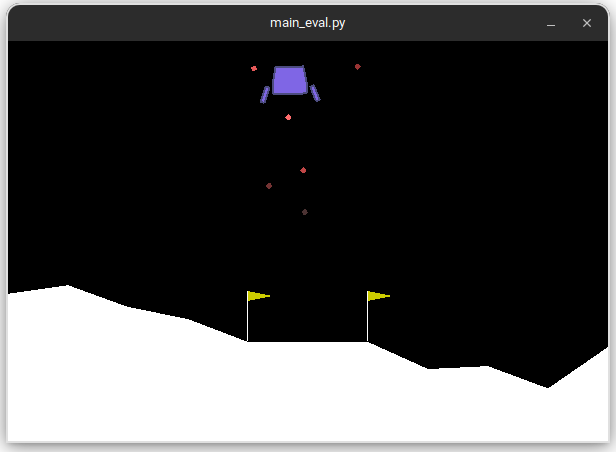
\includegraphics[width=\columnwidth]{./img/lunar-lander-env.png}
    \caption{The Lunar Lander environment.}
    \label{lunar-lander-env}
\end{figure}

\subsection{Acrobot}

\begin{figure}[htb]
    \centering
    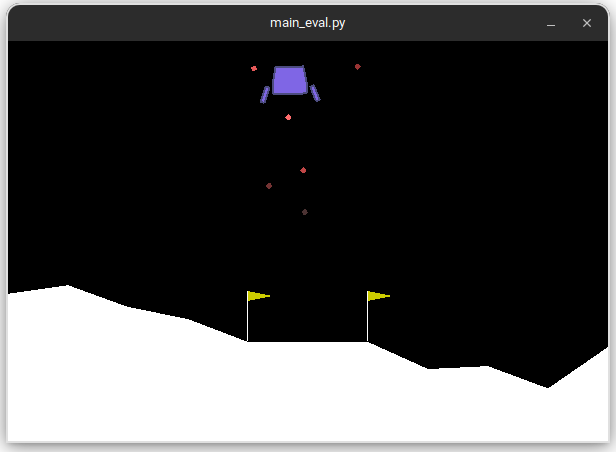
\includegraphics[width=\columnwidth]{./img/lunar-lander-env.png}
    \caption{The Acrobot environment.}
    \label{acrobot-env}
\end{figure}

\subsection{Bipedal Walker}


\begin{figure}[htb]
    \centering
    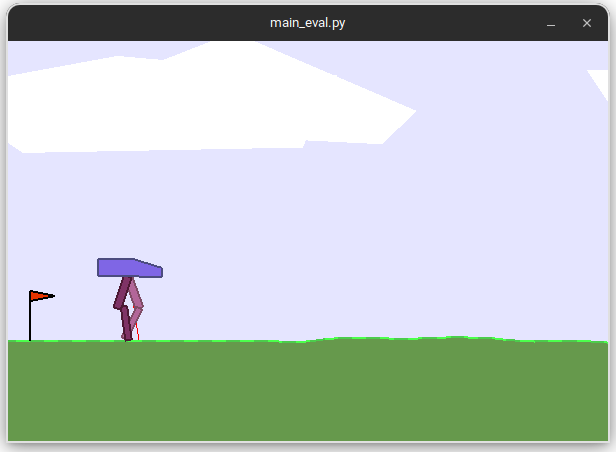
\includegraphics[width=\columnwidth]{./img/bipedal-walker-env.png}
    \caption{The Bipedal Walker environment.}
    \label{bipedal-walker-env}
\end{figure}

%%%%%%%%%%%%%%%%%%%%%%%%%%%%%%%%%%%%%%%%%%%%%%%%%%%%%%%%%%%%%%%%%%%%%%%%%%%%%%%%%%%%%%%%%%%%%%%%%%%%%%%%%%%
%%%%%%%%%%%%%%%%%%%%%%%%%%%%%%%%%%%%%%%%%%%%%%%%%%%%%%%%%%%%%%%%%%%%%%%%%%%%%%%%%%%%%%%%%%%%%%%%%%%%%%%%%%%
\section{Methodology}
\label{sec:methodology}

%%%%%%%%%%%%%%%%%%%%%%%%%%%%%%%%%%%%%%%%%%%%%%%%%%%%%%%%%%%%%%%%%%%%%%%%%%%%%%%
%Reinforcement Learning Methods(5%)
%Describe the reinforcement method/methods you are planning to use in this work. This
%should give the background for the methods. If you are comparing multiple ones, make
%sure to describe them all. Feel free to add diagrams and equations to clarify.

\subsection{Reinforcement Learning Methods}
\label{subsec:reinf-learning-methods}
% PPO, Transformers, GPT

%%%%%%%%%%%%%%%%%%%%%%%%%%%%%%%%%%%%%%%%%%%%%%%%%%%%%%%%%%%%%%%%%%%%%%%%%%%%%%%
%Code Design(5%)
%Describe the general structure of your code including functions, classes, and data struc-
%tures used. If you are using code written by someone else make sure to cite it and
%emphasize the parts that you have written yourself.

\subsection{Code Design}
\label{subsec:design}

%Regarding the code structure employed, we have two main Python files called \texttt{Q\_Learning.py} and \texttt{runEpisode.py}.
%
%The other files are found in the \texttt{rlenv} and \texttt{rllib} folders. The \texttt{rlenv} folder contains the code for the game environment in \texttt{pongclass.py}, while the \texttt{rllib} folder contains \texttt{agent. py}, which contains the code for the Q-Learning and SARSA agents, as well as \texttt{utils.py}, which contains utility functions for parsing command line arguments.

%%%%%%%%%%%%%%%%%%%%%%%%%%%%%%%%%%%%%%%%%%%%%%%%%%%%%%%%%%%%%%%%%%%%%%%%%%%%%%%

\subsection{main\_train.py}
\label{subsec:train.py}


%%%%%%%%%%%%%%%%%%%%%%%%%%%%%%%%%%%%%%%%%%%%%%%%%%%%%%%%%%%%%%%%%%%%%%%%%%%%%%%

\subsection{main\_eval.py}
\label{subsec:eval.py}



%%%%%%%%%%%%%%%%%%%%%%%%%%%%%%%%%%%%%%%%%%%%%%%%%%%%%%%%%%%%%%%%%%%%%%%%%%%%%%%%%%%%%%%%%%%%%%%%%%%%%%%%%%%
%%%%%%%%%%%%%%%%%%%%%%%%%%%%%%%%%%%%%%%%%%%%%%%%%%%%%%%%%%%%%%%%%%%%%%%%%%%%%%%%%%%%%%%%%%%%%%%%%%%%%%%%%%%
%Results Analysis(40%)
%Present the results which answer your hypothesis questions. These should include dif-
%ferent graphs which clarify the answer and examine different aspects of your solution.
%Make sure to carefully describe how your experiments were conducted (how many runs,
%how it was initialized, etc. This section is the most important, and will be evaluated
%both on presentation and correctness.


\section{Results}
\label{sec:results}


%\begin{figure}[htb]
%    \centering
%    \includegraphics[width=\columnwidth]{./img/q-vs-s-running-offline-reward.png}
%    \caption{Q-learning vs. SARSA average offline reward.}
%    \label{q-vs-s-running-offline-reward}
%\end{figure}

%%%%%%%%%%%%%%%%%%%%%%%%%%%%%%%%%%%%%%%%%%%%%%%%%%%%%%%%%%%%%%%%%%%%%%%%%%%%%%%%%%%%%%%%%%%%%%%%%%%%%%%%%%%
%%%%%%%%%%%%%%%%%%%%%%%%%%%%%%%%%%%%%%%%%%%%%%%%%%%%%%%%%%%%%%%%%%%%%%%%%%%%%%%%%%%%%%%%%%%%%%%%%%%%%%%%%%%
%Conclusion(5%)
%What have you achieved in this project? What have you learned?

\section{Conclusion}
\label{sec:conclusion}
\lipsum[2-4]

%%%%%%%%%%%%%%%%%%%%%%%%%%%%%%%%%%%%%%%%%%%%%%%%%%%%%%%%%%%%%%%%%%%%%%%%%%%%%%%
%%%%%%%%%%%%%%%%%%%%%%%%%%%%%%%%%%%%%%%%%%%%%%%%%%%%%%%%%%%%%%%%%%%%%%%%%%%%%%%

% In the unusual situation where you want a paper to appear in the
% references without citing it in the main text, use \nocite

\bibliography{main}
\bibliographystyle{icml2021}

%%%%%%%%%%%%%%%%%%%%%%%%%%%%%%%%%%%%%%%%%%%%%%%%%%%%%%%%%%%%%%%%%%%%%%%%%%%%%%%
%%%%%%%%%%%%%%%%%%%%%%%%%%%%%%%%%%%%%%%%%%%%%%%%%%%%%%%%%%%%%%%%%%%%%%%%%%%%%%%

\end{document}


% This document was modified from the file originally made available by
% Pat Langley and Andrea Danyluk for ICML-2K. This version was created
% by Iain Murray in 2018, and modified by Alexandre Bouchard in
% 2019 and 2021. Previous contributors include Dan Roy, Lise Getoor and Tobias
% Scheffer, which was slightly modified from the 2010 version by
% Thorsten Joachims & Johannes Fuernkranz, slightly modified from the
% 2009 version by Kiri Wagstaff and Sam Roweis's 2008 version, which is
% slightly modified from Prasad Tadepalli's 2007 version which is a
% lightly changed version of the previous year's version by Andrew
% Moore, which was in turn edited from those of Kristian Kersting and
% Codrina Lauth. Alex Smola contributed to the algorithmic style files.
